\chapter{序論}
\label{chap:introduction}

\section{背景}
\label{section:background}
現在、生活が豊かな国では、人間の移動手段は車や電車など交通手段が多様化し、最新技術を駆使した都市化により、座ったまま生活を過ごすことが多くなった。
世界保健機関(WHO: World Health Organization)によると、世界では成人では4人に1人が、そして思春期(11-17歳)の4人に3人が運動不足であり、2型糖尿病、心血管疾患、がん、認知症などの危険性が高まっていると指摘されている。\cite{who_gappa_report_jp}
また、日本では3人に1人が運動不足であり、同じくして生活習慣病、がん、認知症の危険性が懸念される。\cite{obesity_report}
現状、厚生労働省によって3年に1度実施されている「患者調査の概況」では、2017年時点で糖尿病患者数は328.9万人存在しているという報告があり、男性が184万8000人、女性が144万2000人という内訳となっている。\cite{diabetes_statistics}
図\ref{fig:diabetes_total_number}に示すのは厚生労働省の報告書からの抜粋だが、2005年時点で264.9万人、2008年で237.1万人、2011年で270.0万人、2014年で316.6万人、そして2017年時点で最高人数である328.9万人を記録していることが読み取れ、2008年時点で一旦減少したものの、それ以降は年々増加傾向になっていることがわかる。
運動不足による生活習慣病に罹患する人間が増加しており、糖尿病も含め、治療を必要としている人間が多く存在している。

\begin{figure}[htbp]
  \caption{近年における糖尿病患者数の推移(文献\cite{diabetes_statistics}より引用)}
  \label{fig:diabetes_total_number}
  \begin{center}
    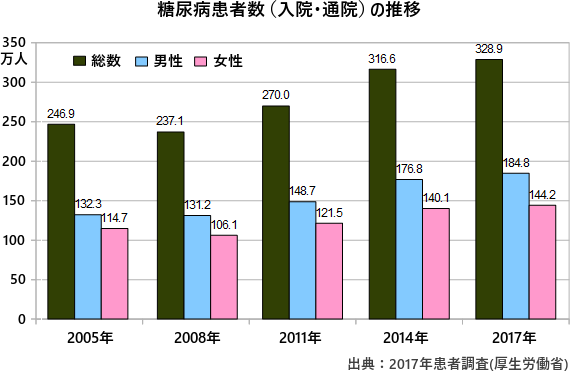
\includegraphics[bb=0 0 600 400,width=15cm]{assets/diabetes_total_number.png}
  \end{center}
\end{figure}

また、病気や疾患の治療では薬物療法が使用される場面が多々ある。入院患者は、看護師などによって薬の服用時間が管理されているが、通院治療の患者の場合それを全て自己管理する必要がある。
薬物療法には、こういった通院患者、自宅治療患者の薬の飲み忘れが問題として存在している。\cite{hokkaido_mc_forget_medicine} \cite{drug_treatment_investigation} \cite{jp_mc_forget_medicine}
日本調剤のアンケート結果では、薬の飲み残しが「よくある」もしくは「たまにある」人が1021人のうち、53.9\%に上り、その中でも「服用するのをつい忘れてしまうから」が65.8\%を占めていた。\cite{jp_mc_forget_medicine}
そして、ファイザー株式会社の、通院治療中の生活習慣病患者(高血圧、高脂血症、糖尿病のいづれか)を対象とした飲み残しアンケート調査によれば、生活習慣病の薬を飲み忘れてしまうことが「よくある」もしくは「たまにある」人が300人の患者の中で46.3\%を占めた。
このように、患者は処方された薬を指示された用法・容量通りに服用することを忘れてしまう場合がある。
これらの問題に対して、現在日本では、朝・昼・夜などの飲みタイミングごとに飲む薬を全て一つにまとめてラベル付けをしておくお薬の一包化、日付や曜日、タイミングごとに飲む薬を分けておくお薬カレンダーや
アプリによる時限式リマインドなどの活用が推奨されている。\cite{jp_mc_countermeasure}

\begin{table}[htbp]
  \caption{処方薬の飲み残しに関する意識調査の結果(文献\cite{jp_mc_forget_medicine}をもとに作成)}
  \label{tbl:forget_medicine_number}
  \begin{center}
    \begin{tabular}{|l||r||r|}
      \hline
      理由  & 回答者数 & \% \\
      \hline\hline
      薬の種類・量が多く飲みづらいから  & 18 & 3.3 \\\hline
      指示通りに飲まなくても良いと思うから  & 60 & 10.9 \\\hline
      体調回復などにより飲む必要がなくなったから  & 165 & 30.0 \\\hline
      副作用が怖いから  & 20 & 3.6 \\\hline
      薬の形状(カプセルや粉薬など)が飲みにくいから  & 6 & 1.1 \\\hline
      服用するのをついに忘れてしまうから  & 362 & 65.8 \\\hline
      薬を余らせておきたいから  & 31 & 5.6 \\\hline
      その他  & 30 & 5.5 \\\hline
    \end{tabular}
  \end{center}
\end{table}

\begin{figure}[htbp]
  \caption{処方薬の飲み残しに関する意識・実態調査の結果(文献\cite{drug_treatment_investigation}より引用)}
  \label{fig:forget_medicine_number}
  \begin{center}
    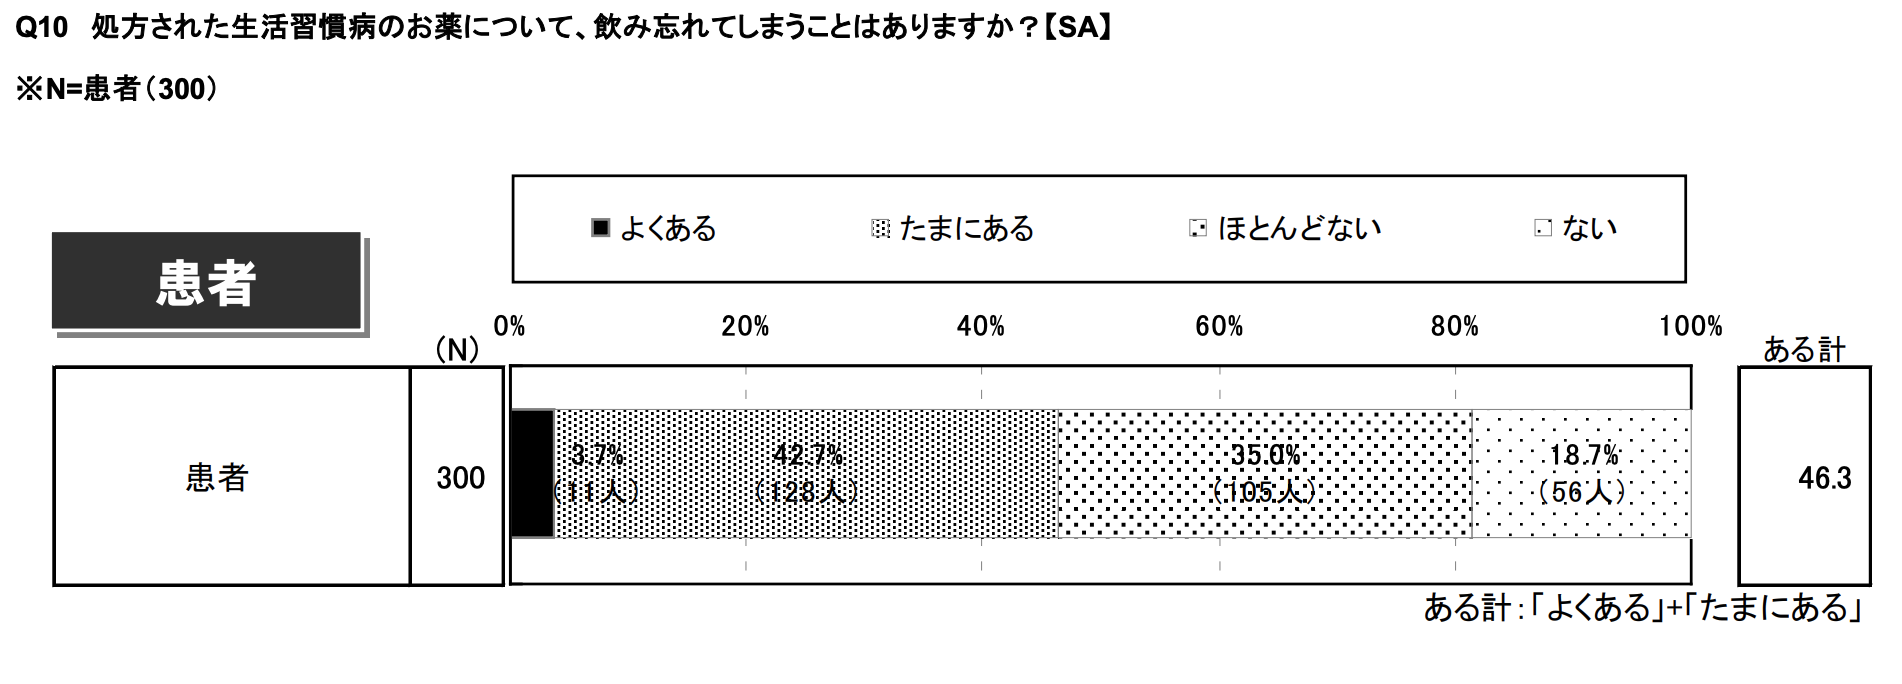
\includegraphics[bb=0 0 1000 400,width=15cm]{assets/forget_medicine_number.png}
  \end{center}
\end{figure}

しかしながら、お薬の一包化やお薬カレンダーは、本人がどこまで正しく飲んだかを知る手段にはなるものの、当人が飲み忘れてしまうことを防止したり、飲み忘れたことを実際に当人が受動的に知る術にはなり得ない。
また、アプリによるお薬アラートは、毎回飲む時間が固定となっているものには有効的であるが、糖尿病患者のインスリン摂取の様な、食事前という時間自体に変動可能性のあるイベントに際したものに対してはその効果は薄いものと言える。

そして、同様に糖尿病治療患者に対しても、インスリン摂取忘れを防止するための試みやプロダクトは様々に提案されている。
プロダクトのインスリンのペン型注射器(以下、「インスリンペン」という。)にキャップとして挿すタイマー\cite{timesulin}や、
アプリと連携したインスリンペン自体がスマートデバイス化したもの\cite{inpen}、
そしてインスリンペンがインスリンを投与したことを自動検知する装着型のデバイス\cite{insulcheck}などが存在している。
これだけのプロダクトが企業から展開されていることからもわかる通り、糖尿病治療におけるインスリンの打ち忘れという課題があることは明確である。

\section{問題意識・対象}

本論文には、糖尿病患者でインスリンを摂取し忘れてしまう人の中でも、看護師や家族からの監視の目がない一人暮らしをしている患者の治療期間の負担を減らしたいという動機がある。
一人暮らしの患者は、第3者による摂取確認には頼れないため、自分で工夫してインスリンを摂取することを覚えておく必要性があり、忘れてしまった時も自分で思い出すことが重要になる。
1日4度訪れるインスリン摂取タイミングの中でも、3回の食前というタイミングを覚えておくのは慣れるまで時間がかかることも考えられるため、他人の助けを借りることができない一人暮らしの患者は
受動的に忘れたことを知らせてくれる何かを持っていることがいくらか助けになる。

\section{本研究で解決したい問題}
\label{section:problem}

本論文では、食前のインスリンを摂取し忘れてしまい、それに気づかないまま食事を行ってしまう患者が、それを知る術がないという問題を解決することを目指す。
図\ref{fig:insulin_4times_method}に示したように、この4回法と呼ばれる治療法は、1日の中で、4回のうち3回は毎食食べる直前にインスリンを摂取する必要があるが、これは当然のことながら患者が自主的に投与を行う必要がある。
もし生活習慣が安定しており、朝食、昼食、夕食の時間が常に定まっている場合は、その時間に合わせてタイマーを設定して自分にリマインドする、という手法をとることでインスリン摂取忘れを防ぐことは可能である。
しかしながら、通院と在宅治療を行う多くの場合、食事時間が定まっておらず、その設定された時間が、必ずしもインスリンを摂取すべき時間であるとは限らないのが現実である。
また、別居もしくは同居している家族から定期的に確認してもらうという手法も考えられるが、これも属人的な手法であり、そのタイミングはまちまちであるため、摂取を忘れたまま食事をしたという事実に基づいた通知ではないため、問題の解決策として不安要素が残る。

このように、在宅での治療では、インスリン摂取の確実性が担保できず、また忘れたこと自体を知る術もないため、その後の担当医師への連絡や対応が遅れてしまう可能性がある。
そして、この問題を解決するためには、以下の2つのタイミングを把握し、適切に患者に対してフィードバックを行うシステムが求められる。

\begin{enumerate}
  \item 患者のインスリンを摂取した時間
  \item 患者が食事を開始した時間
\end{enumerate}

本論文では、これら上記の2つの時間を使い、食前のインスリン摂取を忘れた時に糖尿病患者に知らせることを可能にすることを目標としている。

\section{目的}
\label{section:purpose}

糖尿病患者がインスリンを投与し忘れた場合、気づき次第打ち忘れた分を服用するのではなく、担当医に連絡をした上で指示を仰ぎ、適切な量のインスリンを適切な時間に摂取する必要がある。
つまり、患者自身が自分が忘れていることを認知さえすれば、その後の迅速な対応をすることが可能である。

そこで本論文では、食事やインスリン投与というイベントをトリガーとした、インスリンの服用し忘れを治療患者に知らせ、糖尿病治療におけるインシデントを減らし、援助するためのツールを提案することを目的としている。

また、食事の検知にはカメラ映像と画像認識技術を使用した研究があるが、被験者にとって常に撮影されているという煩わしさは、家庭での導入を考えると現実的ではない。
他にも、顎や腕に直接装着する形のウェアラブルデバイスを用いた食事検知の研究がなされているが、こちらも常に体に装着しておかなければならないことは当事者にとって動き辛さなどに繋がり、制約になってしまう。
本研究では、上記にあげたような制約を可能な限り取り除いた上で、インスリンが実際に摂取された時間と、食事を開始した時間を取得し、糖尿病治療中の患者をサポートするためのツールの提案を目指す。

\section{本論文の構成}
\label{section:structure}
本論文における以降の構成は次の通りである。
\ref{chap:diabetes}章では、本論文を読む上で補助となる、糖尿病や、その治療に関する前提知識を述べる。
\ref{chap:related_works}章では、本論文に関連する研究やプロダクトを紹介し、それぞれの特徴とそれらと本研究との差異を示す。
インスリンデバイス、加速度による行動検知、そして食事開始の検知と、幅広く関連研究をあげている。
\ref{chap:design}章では、加速度センサーによる食事検知とインスリンデバイスによるインスリン摂取忘れを通知するためのシステムの設計について述べる。
\ref{chap:implementation}章では、\ref{chap:design}章で述べた内容の実装に用いたライブラリや実モジュールに言及しながら詳細な実装内容について述べる。
\ref{chap:evaluation}章では、\ref{chap:implementation}章で実装したインスリン摂取忘れ通知システムの評価を行い、その結果について考察する。
\ref{chap:conclusion}章では、本論文のまとめと今後の展望について述べる。
